\section*{Abstract}
The main goal of this project is to explore and examine the properties of 802.11. Wireless security is critical to maintain internet infrastructure and is therefore the focus of both hackers and network administrators. WEP was one of the first ways to encrypt wireless data, but has glaring flaws in its algorithm. Even with good encryption many wireless networks are vulnerable to deauthentication attacks. In this project we have cracked the password for WEP access and shown that by just capturing packets from a single user on an AP, we can decrypt all data that has been sent over that connection. We have also created a WiFi-scanner in connection with our deauthentication attacks that show key information on local wireless local area networks. A deauthentication attack has been successfully completed on a modern device. This shows that even secure networks using technologies in use today, are still at risk of certain attacks. 

\newpage
\tableofcontents
\newpage

\section{Introduction}
Wireless security as become increasingly critical due to the rapidly expanding use and need for internet access. Many devices use WiFi to connect to the internet, such as smartphones and laptops. As data over WiFi is sent via radio waves and thus uses a shared medium there is a coherent risk. The data is at risk of being captured by bad actors and is prone to manipulation. Thus a need for strong encryption and control of ones data is necessary. However, even with security measures in place for wireless networks, there's and are still vulnerabilities to attacks on said networks. One such attack, which is the focus of this report, is a denial-of-service attack: the deauthentication attack. It's an attack where a user will be rejected access to the network and thereby either disrupt a workplace or pave the way for other more sophisticated attacks such as the Evil Twin Attack.

This project will explore the theory and practical applications of deauthentication attacks on networks. Further we will explore password cracking for passwords used in the encryption of wireless network traffic using the now outdated WEP protocol. To achieve these goals information about the wireless local area network (WLAN) has to be known. Therefore another goal for the project is obtain information of available SSIDs, clients connected, signal strength and so on.

When this project is done, we hope to have explored the the theory and practical applications of deauthentication attacks on networks and the building blocks that make up data-packets in a wireless network. It is important to note that this project is for educational purposes only and should not be used for malicious activities.

\section{Functionality}
Our project constists of the following functionalities:
\begin{enumerate}
    \item Scan the WLAN and identify key information about clients/Access Points
    \item Perform deauthentication attack on WiFi devices
    \item Capture packets and obtain clear text by Password cracking of WEP
\end{enumerate}

These functionalities aim to be the core of the product that will be created. The first functionality, scanning for local networks, is the most important one as that is the basis of all other functionalities.

A deauthentication attack is a type of denial-of-service attack that targets communication between a user and a WiFi wireless access point \cite{Deauth}. It exploits a feature of IEEE 802.11 wireless networks that allows devices to disconnect from a network by the deauthentication management frame \cite{Deauth_Wiki}.
A deauthentication frame tells a device to stop using communication with the AP. It can be sent by either the AP or the device itself. It's normally used for legitimate purposes, such as ending a connection or switching to another network (handover). Yet there is no identification check performed in this procedure. Hence an attacker can exploit this feature and send deauthentication frames to the AP with a spoofed client source address. This causes the connection to close making the spoofed device's connection end and probably reconnect. This exploitation has multiple use-cases. If done repeatedly or to multiple devices, this can disrupt or disable the network entirely, thus resulting in a Denial-of-Service (DoS) Attack. Meanwhile it can also be used to obtain a EAPOL 4-way-handshake for WPA or as a way to misguide a client to a rogue access point created by a malicious user to obtain a Man-In-The-Middle state, known as an Evil Twin Attack. 

The last point is password cracking. The product should be able to crack/obtain the WiFi-password in the WEP algorithm. The WEP is one of the most basic WiFi algorithms. It is an outdated and non secure algorithm and the product utilizes  Aircrack-ng's PTW method to recreate the passkeys on the AP's \cite{aircrack-ng}. The method needs data-packets from users on the network containing initialization vectors and those are captured by WiFi scanner as that is it's primary functionality. When the scanner has gotten enough packets, around 10.000, it will give those to the password crack which then finds the passkeys using Aircrack-ng. This part utilizes a tool already known, thus the greater focus here will be theoretical.

The implementations are mainly based on the python library Scapy\cite{scapy} to implement the functionalities. As our network interfaces has to be put in monitor mode a UNIX environment is used. The longterm goal is to use a raspberry pi later to obtain mobility and a uniform platform. 
The network interface is a Realtek DWA 131-E1 dongle as it is cheap and allows for monitor mode. The UNIX platform has the consequence of limiting the use of the implementation to a specific operating system. Though this should be able to be ported to Windows and MacOs if need be. Here the Linux-sub-system (WSL) on Windows might be exploited.
The positive side of using UNIX is that we can implement the program on many types of systems as we use a virtual machine to create the product. Thus making conversion to a raspberry pi easier. The negative side is that we have to use a virtual machine which can create problems with drivers and performance. 

\subsection{Mapping of networks}
This block takes the physical data being sent in the wireless space, and transforms it into information that the other blocks need and use. It contains a table that holds the information as sub-blocks, for instance access points in the WLAN, as well as the clients on said AP. Or the signal strength of the AP and which channels are used. This mapping can be done via beacon management frames used by APs to announce their respective presence. Likewise probe management frames can be used to understand what APs a client has been associated with in the past.
The block also contains a way of collecting data-packets containing initialization vectors and sending them to the password cracking block. 

\subsection{Deauthentication}
This block handles deauthentication, wherein we deny clients access of certain AP's or all wireless internet usage. Thus making the sub-blocks: 
\begin{itemize}
    \item Client
    \item AP
    \item Channel
\end{itemize}


\subsection{Password cracking and WEP/WPA2}
This block handles the actual cracking of WEP from data-packets collected from the mapping block. The data should be combined into a single file which can then be analysed and the password/passkey found.

\section{Theory}
The primary conceptual framework underpinning this project revolves around the 802.11 standard \cite{IEEE802.11}. The 802.11 standard is a set of wireless network protocols developed by the Institute of Electrical and Electronics Engineers (IEEE). The first version of the standard, 802.11, was released in 1997, and since then, several revisions and amendments have been made to improve the technology and increase its capabilities \cite{ETHW}.

The 802.11 standard uses radio waves to transmit data between devices within a WLAN without the need for cables or wires. This makes it a popular choice for connecting mobile devices to the internet, especially in homes, offices, and public places such as cafes, airports, and hotels \cite{Public_WiFi}.

Throughout the project, programming will be done mainly in python, using the library Scapy for sniffing, analyzing and transmitting packets. Scapy is a program written in Python, that gives the ability to construct, decrypt, send, capture packets and much more \cite{IEEE_Scapy}. Scapy gives us tools for analyzing 802.11 frames, thus providing the information contained in 802.11 frames. Packets in Scapy are created as objects with layers built on top of each other to define the type of the packet.
\\

\begin{figure}[!htbp]
    \centering
    \includegraphics[width=0.5\textwidth]{Latex-Files/Billeder/WiFi_Types.png}
    \caption{WiFi typer og subtyper}
    \label{WiFi Types}
\end{figure}

There are 3 frame types in 802.11: Management-, control- and data-frames \cite{Amit802.11frames, DefinitiveGast}. Figure \ref{WiFi Types} shows some of the types and subtypes of different frames with a focus on management frames, since that is what our project is focused on.  Management frames are used by AP's to join and leave the basic service set (BSS). They have a MAC header, a frame body, and a trailer. These frames are needed because it is difficult to connect to a wireless network compared to a wired network. With a wire you mostly just need the physical connection where data can only flow between the user and the router. With a wireless connection, all data is sent everywhere and each router and user needs to know which data-packets to ignore and which to receive. This is done via management frames where a user associates with an Access Point (AP) and agree on conditions, like security and speed. For a user to know which AP's are near, it needs to scan the surrounding area. This is done via 2 ways of scanning: Active scanning and passive scanning.

In passive scanning each AP broadcasts beacon frames and a user sends an association request to the AP it wants to connect to. In active scanning the user broadcasts probe requests and each AP responds to this request with a response back to the user. When the user then wants to connect to an AP that has responded it sends an association request to that specific AP. 


\subsection{WEP & WiFi security standards}
Wireless networks also need security while sending packets, i.e. authentication and confidentiality. To ensure confidentiality data frames are encrypted with some sort of security standard. The oldest widespread type being Wired Equivalent Privacy (WEP). It had major security flaws that allows hackers to bypass the algorithm and read the data being sent \cite{WEP1}. Therefore was WiFi Protected Access (WPA) developed in 2003 \cite{WEP3}. 

WEP uses a secret key to encrypt packets between client and AP \cite{WEP2}. The problem with this is that WEP uses the RC4 encryption algorithm, which is known as a stream cipher. A stream cipher operates by making a short key into an infinite random key-stream. The client uses XOR on the key-stream with the plain data to produce the encrypted data. The AP has a copy of the same used key, and uses it to generate an identical key-stream. The AP then uses XOR on the key-stream with the encrypted data to get the exact same plain data back. This type of encryption is easy to misuse, since by flipping a single bit in the encrypted data, the plain data will also have a corresponding single bit flipped. Also the XOR can be found via statistical analysis of key-streams to thereby recover the plain data.

\begin{figure}[!htbp]
    \centering
    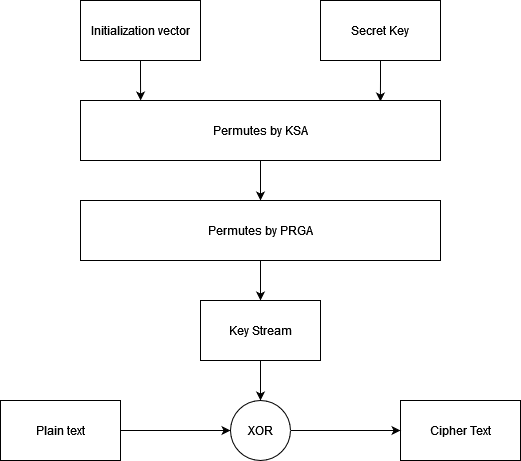
\includegraphics[width=0.4\textwidth]{Latex-Files/Billeder/RC4.png}
    \caption{Simplified RC4 algorithm \cite{geeks}}
    \label{RC4}
\end{figure}


WEP has incorporated defenses against these 2 types of attacks, but they are implemented poorly. The defense against flipping bits are integrity checks in the packet implemented as a CRC-32 checksum. Sadly it is linear which means that it is possible to find the difference between 2 CRC's because the bits that are flipped in the encrypted data is deterministic and therefore an attacker can adjust the checksum and then it is believed that the integrity of the packet is kept, when in reality it isn't.

The defense against the statistical attack is an initialization vector to decrease the chance of reuse of key-streams. The vector is only a 24 bit field and that guarantees the reuse of key-streams because the vector was too short and when thousands or millions of data-packets are sent, reuse will happen quickly. It would take around 110.000 data-packets to ensure reuse \cite{Random_map}. Because of this, the attacker can easily pick up enough data to perform statistical analysis of packets using the same key-stream and then recover the plain data.

Fortunatly mitigations for WEP flaws is already industry standard by the WPA2 protocl, which was a development of the intermediate measure WPA, as a security update to fix many of WEP's problems \cite{WPA2_1}\cite{WEP3}. It was released in 2004 in the 802.11i amendment to the original 802.11. WPA2 uses CCMP protocol which is a development of the AES security algorithm. It rids the network encryption of the previously mentioned security vulnerabilities. 
\\
\begin{figure}[!htbp]
    \centering
    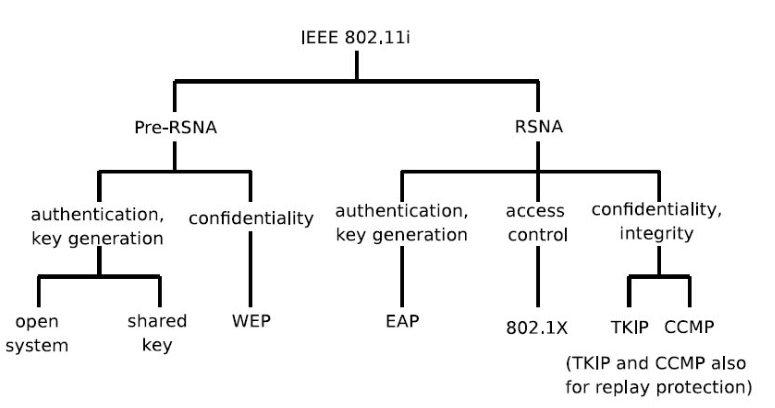
\includegraphics[width=0.6\textwidth]{Latex-Files/Billeder/802.11i security.png}
    \caption{Summary of 802.11i security \cite{WPA2_3}}
    \label{802.11 Security}
\end{figure}

Figure \ref{802.11 Security} shows the different types of securities in the 802.11i standard. It is split up into pre-RSNA and RSNA. RobustSecurity Network Association (RSNA) is the way to describe the updated security protocols established with 802.11i and basically means that all security before this standard is out of date. 

For a product to be WiFi certified it requires the usage of a modern security protocol, which is WPA2 \cite{WPA2_2}. New security vulnerabilities have since been found in WPA2 and WPA3 has been created to solve some of those, WPA3 is planned to be implemented widepsread soon. Our focus is not to try decrypting WPA2 or WPA3. 

\subsection{Deauthentication in WLAN}
The authentication of clients and AP's can be exploited by deauthentication attacks. The theory behind this attack is based on the 802.11 standard, which allows clients to disconnect from an AP using a deauthentication frame.

When a client device is connected to a WiFi network, it sends periodic beacon frames to the access point to maintain the connection. In a deauthentication attack, an attacker sends a series of forged/spoofed deauthentication packets to the target client or AP, pretending to be the legitimate access point or client. This causes the target to disconnect from the network and require reauthentication, disrupting the communication between the client and the access point.

Deauthentication frames are frames of the management type as seen in figure \ref{WiFi Types}, and have the overall structure as such. Therefore the deauthentication frame contains, among other things, 3 addresses. These addresses being the destination address, the source address, and the BSSID of the AP's wirelsess interface, the address of the AP  These three addresses are what can be altered in order to perform a deauthentication attack. One field of in a deauthentication frame is the reason code which is 16-bit, this defines the reason for the termination of the connection. There can thus be upwards of 65535 reason codes, yet about 66 is utilized \cite{Cisco_Deathentication_reasoncodes}. Apart from a reason code, the frame body includes vendor specific elements, and the Management MIC IE(MMIE) \cite{IEEE_802.11w}. Though this is not always present. 

802.11w, released in 2009, introduces protected management frames thereby combating attacks such as deauthentication attacks. This is achieved by ensuring the integrity in the management frame. The integrity check is achieved by the sender calculating a message integrity check(MIC) value, and appending this to the frame. The receiver then calculates the MIC value using the same algorithm, and compares the two. If the two MIC values match, the frame is considered to not having been tampered with, and thus marking it as authentic. Furthermore a frame sequence number(FSN) is introduced, which is used to prevent replay attacks. Replay attacks are not something we will be covering in this project and therefore it wont be analyzed in this report. 
The MMIE is thus only in use when protected management frames are enabled \cite{IEEE_802.11w}. Protected management frames were introduced in order to combat the deauthentication attack. Since the deauthentication frames without protected management frames has no integrity check by nature, this creates a sizeable vulnerability for a network as attacks such as the deauthentication attack can be exploited.

\section{Implementation and tests}

\subsection{Mapping of networks}
As established WiFi utilizes a shared medium and even though the data send generally is encrypted some data has to be send in clear text. The header contains a lot of information needed for the communication system to be established and working. This can exploited as well to do reconnaissance of the WLAN. As data is transferred freely over the medium it is also possible for devices on the medium to "listen" to others communication - hence the implementation will exploit passive scanning, thus not participating in the communication but rather analyze and save essential data from the traffic. The point of this implementation is to gather information about APs and the associated clients. The logic for this implementation is showed on figure \ref{} as a flowchart.




\subsection{Deauthentication}
Our implementation of the deauthentication functionality relies on the ability to create and send packets with the use of Scapy. Thereby forging our own deauthentication frame, thus gaining the ability to set our own parameters for the packet.
As shown in figure \ref{deauth_prompt_code}, our implementation of the deauthentication as follows. 
The user is first met with a menu of the known AP's that are eligible for attempting an attack. The know AP's are all found using our mapping of the network.
we have then decided to show another prompt menu which gives the user the option of choosing the target from a list of the already known clients if so desired. If not the user can either input a MAC-address, or choose to use the broadcast address, resulting in all clients receiving the deauthentication frames. 

\begin{figure}[!htbp]
     \centering
     \begin{subfigure}{0.49\textwidth}
         \centering
         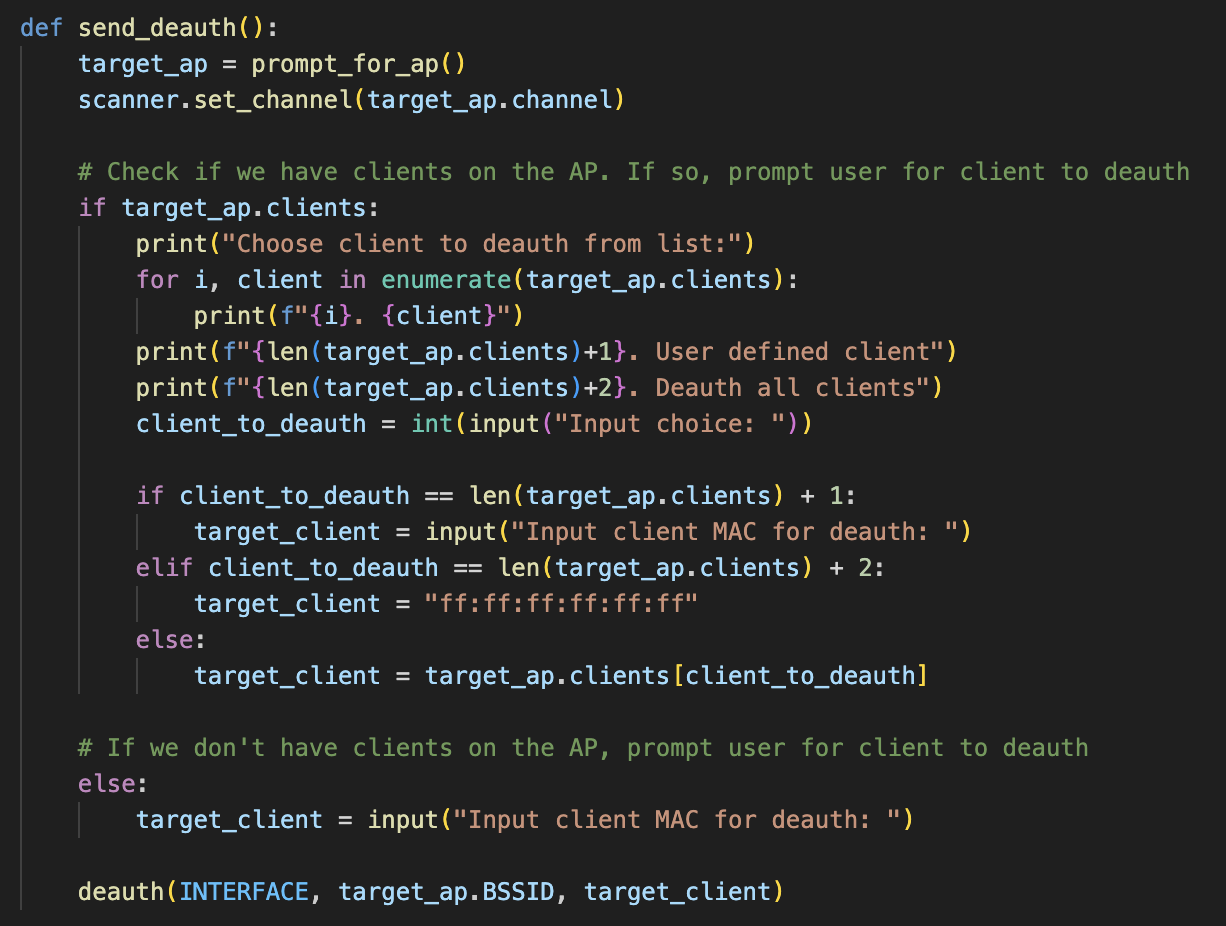
\includegraphics[width=\textwidth]{Latex-Files/Billeder/deauth_prompt_code.png}
         \caption{Code for prompt and call of attack}
         \label{deauth_prompt_code}
     \end{subfigure}
     \hfill
     \begin{subfigure}{0.49\textwidth}
         \centering
         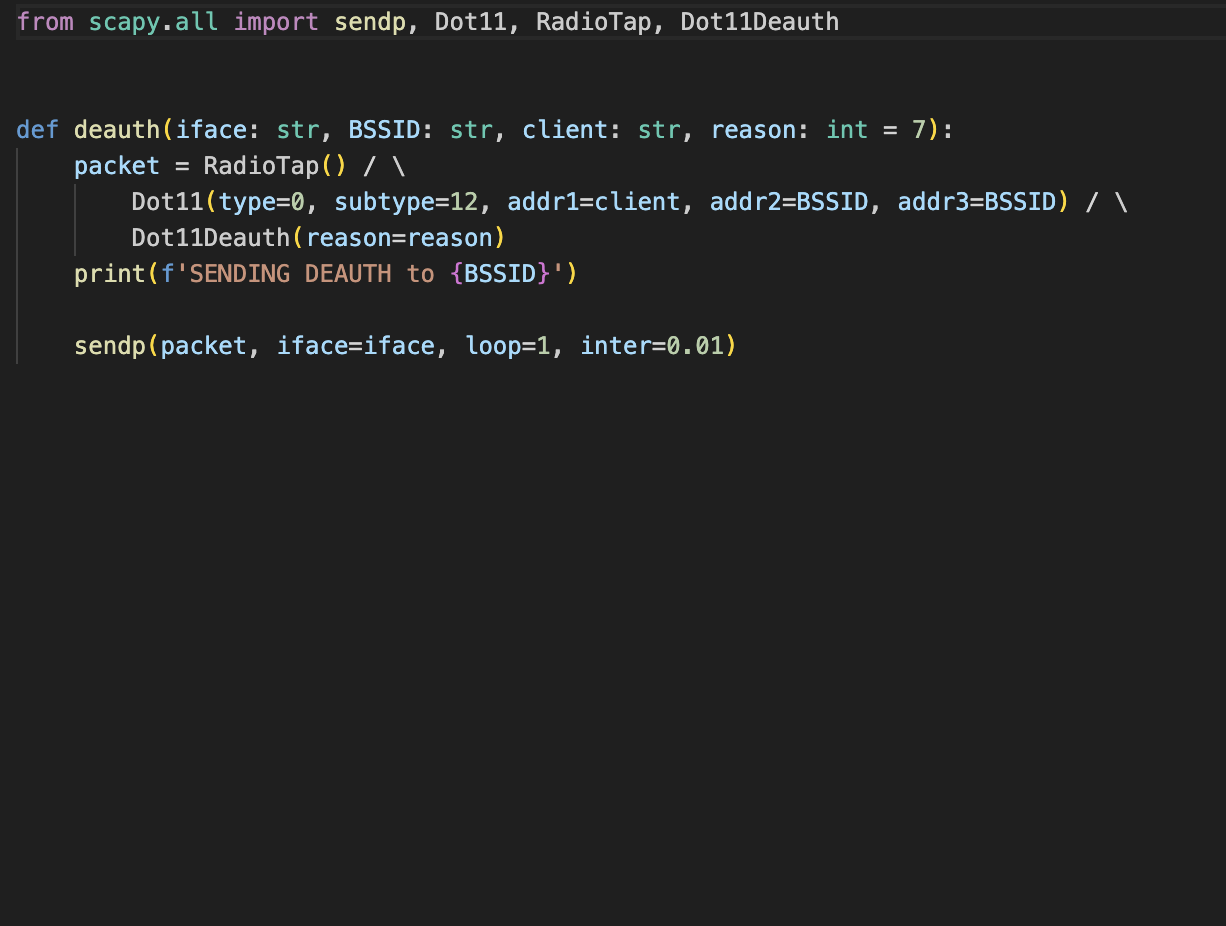
\includegraphics[width=\textwidth]{Latex-Files/Billeder/deauth_func_code.png}
         \caption{Code for deauthentication attack function}
         \label{deauth_func_code}
     \end{subfigure}
     \hfill
     \caption{}
\end{figure}

After a target AP, and a target client has been defined, the "deauth" function, seen in figure \ref{deauth_func_code}, is then called. This function is what creates the appropriate deauthentication frames. The instantiating of the packet works by stacking layers on top of each other. In this case the packet is created by first making a RadioTap layer, which is responsible for sending the packet we create.
Then a Scapy "Dot11" layer is made, which represents a basic 802.11 frame. Here we set the type to 0, indicating a management frame, and the subtype to 12 indicating a deauthentication frame. From here the addresses are defined for the target of the frame. Finally the last layer is added, this being the "Dot11Deauth" layer which here defines a reasoncode for the deauthentication. This reasoncode is set to be 7 for default, which corresponds to the reason "Class 3 frame received from non-associated STA"\cite{Cisco_Deathentication_reasoncodes}. In a communications relation, the reasoncode provides important information about the cause of the deauthentication. However it is not an integral part of the deauthentication action itself, therefore the reasoncode is just given as a random number we have chosen.
Although it does not have a functional use, the reasoncode could in practice improve a deauthentication attack, by using appropriate reasoncodes, thus further concealing the fact that it is of malicious nature.
Subsequently a line is printed to the console notifying the user that a deauthentication attack will commence, combined with the target for the attack.
Ultimatly the "sendp" function, sends the beforehand created deauthentication frame.

\begin{figure}[!htbp]
     \centering
     \begin{subfigure}[b]{0.49\textwidth}
         \centering
         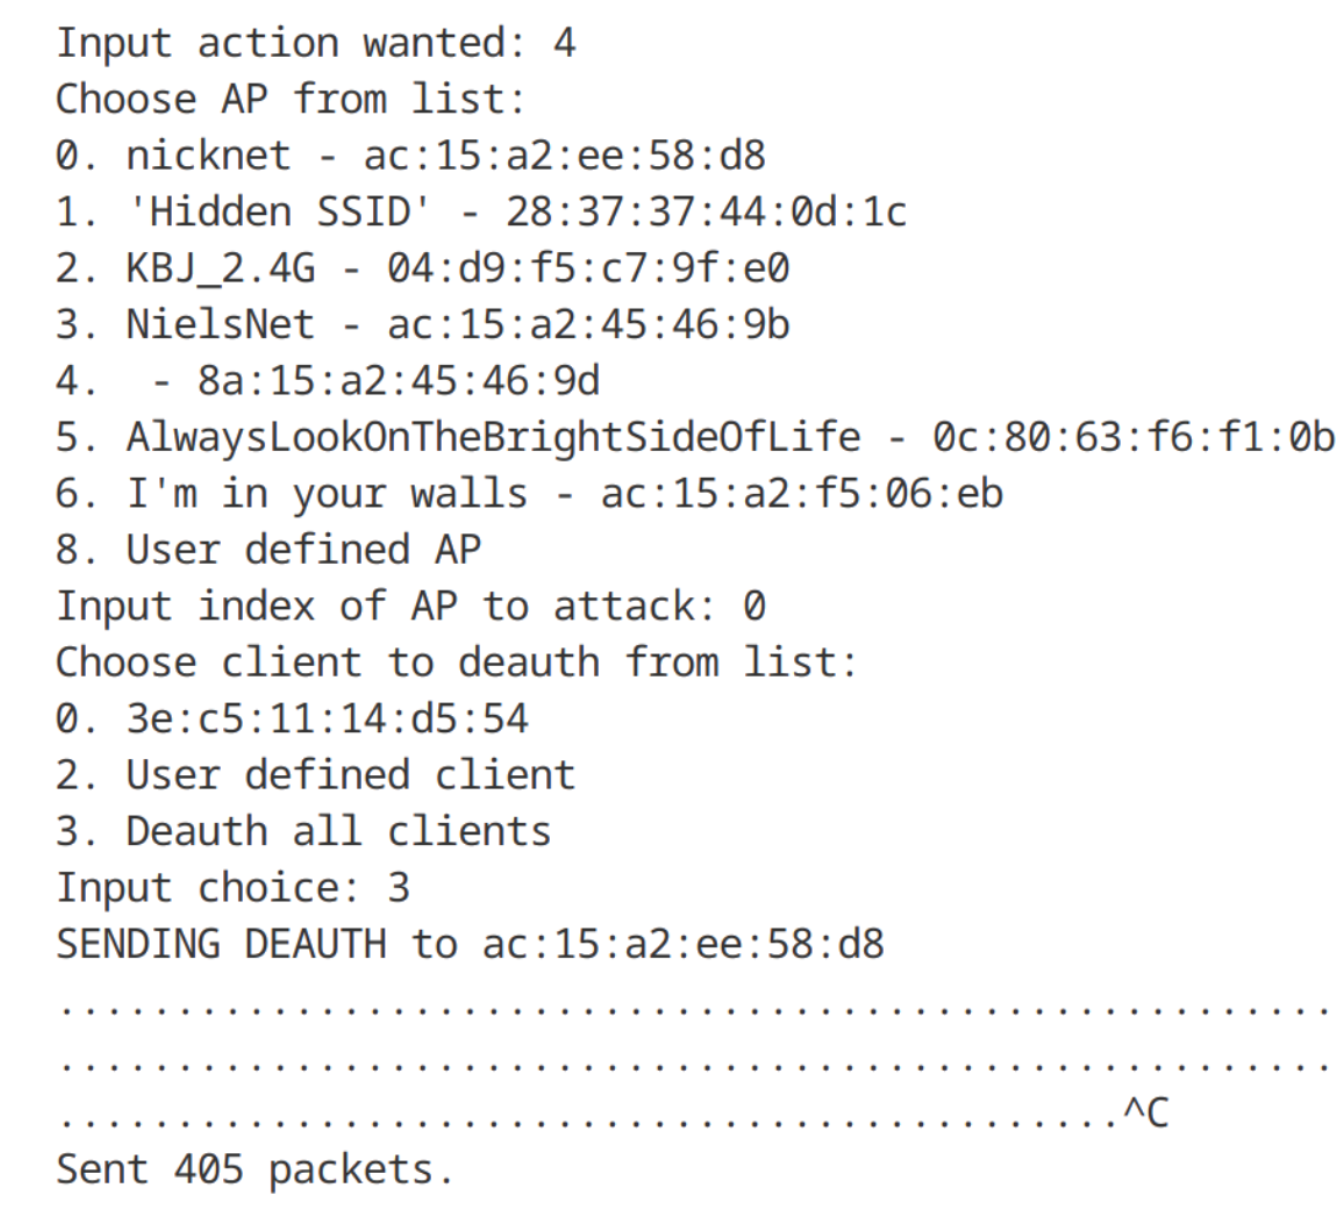
\includegraphics[width=\textwidth]{Latex-Files/Billeder/deauth_attack.png}
         \caption{Output when running deauthentication attack}
         \label{deauth_attack}
     \end{subfigure}
     \hfill
     \begin{subfigure}[b]{0.49\textwidth}
         \centering
         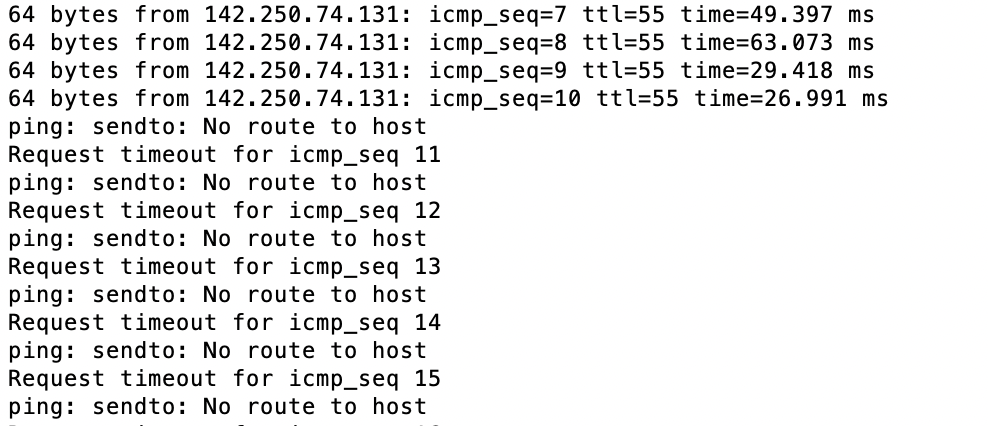
\includegraphics[width=\textwidth]{Latex-Files/Billeder/deauth_ping.png}
         \caption{Result from being attacked (Mac)}
         \label{deauth_ping}
     \end{subfigure}
     \hfill
     \caption{}
\end{figure}

Figure \ref{deauth_attack} shows the output presented to the user, when performing the deauthentication attack. The user can here choose to selectively deauthenticate a single client. Alternately the user possesses the option to deauthenticate all clients from the targeted access point. Upon the user inputting a choice, the program begins transmitting the packet constructed. The deauthentication attack is continuous and will only stop when interrupted by the user. 
Figure \ref{deauth_ping} shows the result from our deauthentication attack on a Macbook connected to a mobile phone hotspot. This attack was run by deauthenticating a single client. it is evident that the pinging to google works in absence of complications, however when the deauthentication attack is deployed, the pinging encounters issues and outputs "No route to host". Thereby denying the client service, and disconnecting the client from the internet. 
Figure \ref{deauth_ping_windows} shows a similar attack on a Windows PC.

\begin{figure}[!htbp]
    \centering
    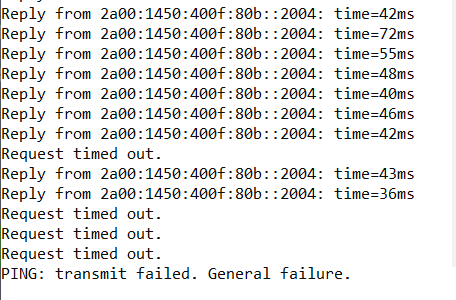
\includegraphics[width=0.5\textwidth]{Latex-Files/Billeder/Deauth virker.png}
    \caption{Result from being attacked (Windows)}
    \label{deauth_ping_windows}
\end{figure}


Our deauthentication implementation has undergone limited testing, highlighting the need for further investigation. Our objective is to assess its functionality in various scenarios, including both successful and unsuccessful cases. Furthermore, we aim to evaluate the performance of the code by conducting tests on edge cases. Additionally, we plan to examine the behavior of the implementation when multiple clients are connected, observing whether all of them are successfully deauthenticated. 


\subsection{Password cracking}
A test has been successfully done where, using Airodump-ng for capturing packets, a network has been cracked and the password found. 

\begin{figure}[!htbp]
    \centering
    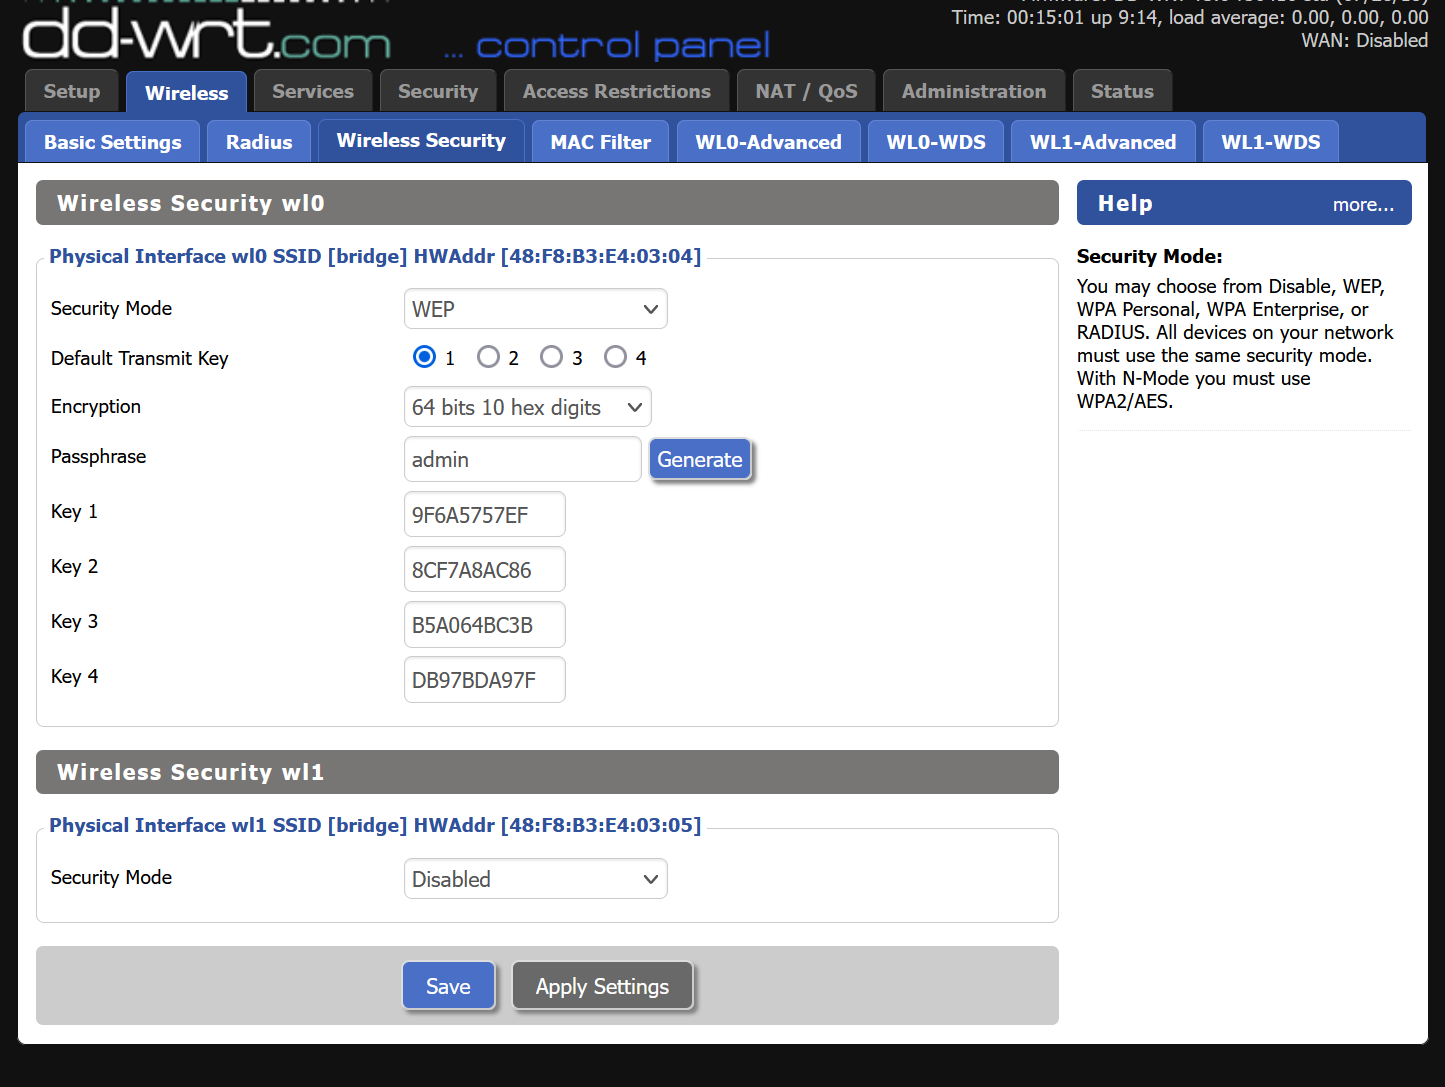
\includegraphics[width=0.5\textwidth]{Latex-Files/Billeder/Kode2.png}
    \caption{The passwords on the AP}
    \label{Crack2}
\end{figure}

The test was that an AP, with the capability to use WEP, was set up and connected to a wider network on the internet and then made to use WEP with passkeys, as seen on figure \ref{Crack2}. Then a computer using Linux was connected to that AP and a constant stream of data was created by watching YouTube. Then another computer was setup to monitor these data-packets and capture those that contain an initialization vector (IV). 

There was a small problem with the connection between the AP and the wider internet, so we had to constantly pull the ethernet plug and replug. This was probably because the wider network didn't like using WEP, and that was also why YouTube did not actually work. So the computer sent and received data-packets from the AP only. Enough data-packets where still created and so a large .pcap file was made with about 10.000 IV packets. 

\begin{figure}[!htbp]
    \centering
    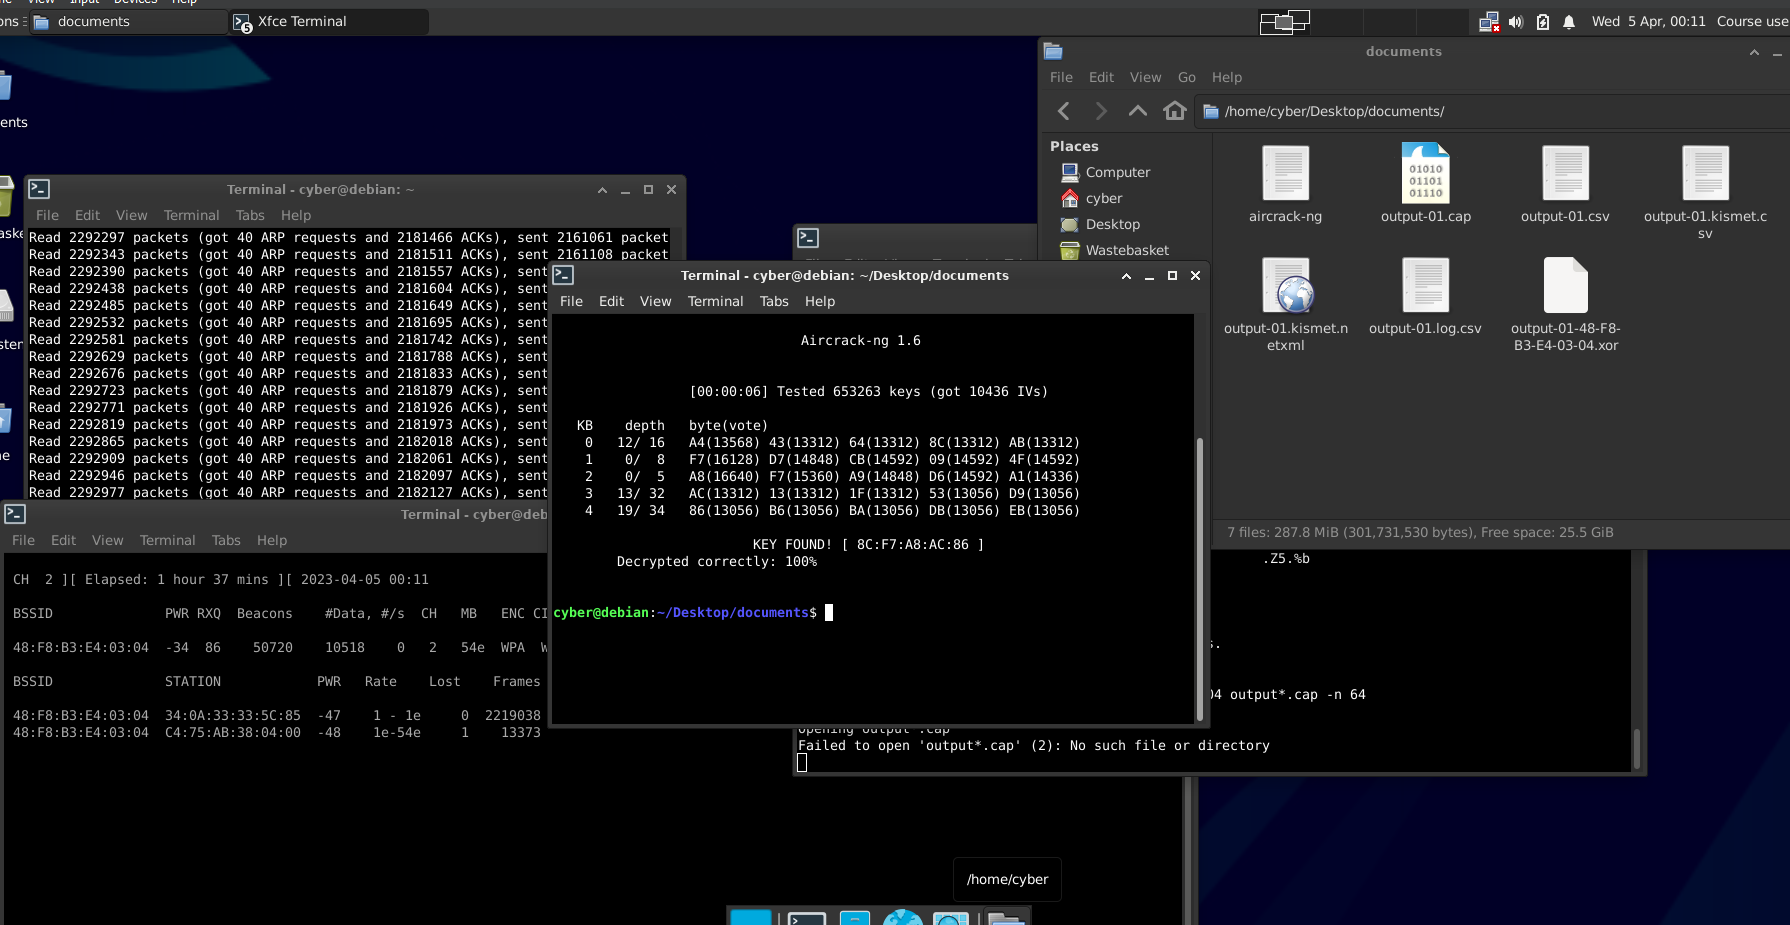
\includegraphics[width=0.5\textwidth]{Latex-Files/Billeder/Kode1.png}
    \caption{Aircrack-ng finding the password}
    \label{Crack1}
\end{figure}


Then Aircrack-ng was used on this .pcap file to find the passkey, which it did after 6 secounds. The passkey corresponds with one of the chosen passkeys on the AP. We can see the result on figure \ref{Crack1}.

Hopefully we can capture packets containing IV's using the WiFi-scanner and Scapy and place them in a combined file. That would make it simple to crack the WEP algorithm using Aircrack-ng and thereby recreating the passkeys and allowing access to the data-packets. 

\section{Main Challenges}
Our main challenge in this project is the fact that internet traffic is complicated and made up of many interlocking parts. There is a lot of data being sent constantly and most of it is not relevant to what we are doing. As we are working with a shared medium it can be hard to differentiate between what we are creating and what is part of the standard traffic. That makes it difficult to figure out what is going on 'under the hood' when testing our implementations. Thus it has so far taken much longer to perform some of the basic steps of mapping the network and simple deauthentication. Still this is very much a learn by doing project in the way that we obtain solutions to either tackle or overcome the obstacles and after implementing our WiFi-scanner we have gained valuable knowledge about how data-packets are built. 

Likewise the theory behind most of the 802.11 management frames and such used in this project is very new to us, since only a short overview of 802.11 has been provided in our courses where the focus mainly has been on the EAPOL 4-way-handshake within WPA. Thus there is a great gap in knowledge we need to fill as some of the implementation parts require a deep understanding of how e.g. the procedure for deauthentication works.

When cracking WEP, the main challenge is figuring out how to create enough packets consistently that contain IV's and are use the same passkey. Also if this is successfully implemented we also have to recreate Aircrack-ng's PTW method to crack the WEP algorithm. Then this needs to be integrated with the rest of the code. 

\section{Timeplan}
This is the current timeplan for the 3-week period. We are planning on writing on the report concurrently with working on the implementation and tests. We are probably not working on the report every day, but at least multiple times a week. We have set time off for the last week to work on the presentation and on the report to finish it and that we should be done with coding at this time. 
\begin{figure}[!htbp]
    \centering
    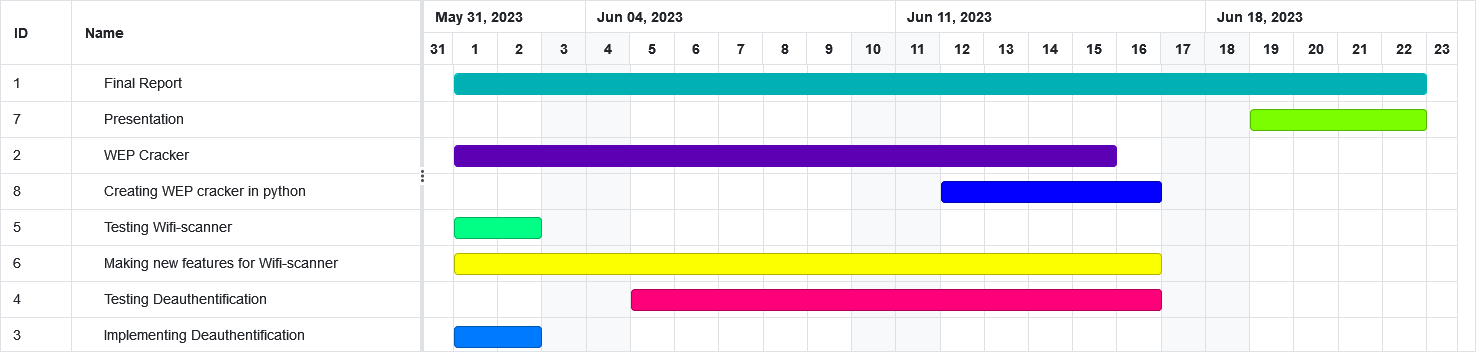
\includegraphics[width=1\textwidth]{Latex-Files/Billeder/Online Gantt 20230530.png}
    \caption{Timeplan}
    \label{timeplan}
\end{figure}

\section{Conclusion}
In this project we have investigated network traffic by mapping local WiFi networks using python and the tool Scapy to show all AP's connected and sending beacon frames and the clients connected to these networks. We also did deauthentication attacks to disconnect one or more clients from using wireless networking. By doing this we gained advanced knowledge about different types of frames and subframes in the 802.11 standard. We also investigated security in the 802.11, namely WEP. During this project we also increased our knowledge of python programming and networking toolboxes that use python, which gives a broad understanding of how packets are built in python and in general. 



